After being cleaned, the bearings will be filled with high-quality mineral oil, free of acid and not too fluid.
Before filling, close the drain hole and unscrew the overflow plug located on the side of the bearing.
Pour the oil into the bearings until it overflows from the overflow, which will then be closed with its plug.
The overflow level should not be exceeded, as excess oil may flow into the motor, or the lubricating rings will remain stationary.
Ensure that the rings rotate and stir the oil.

Ball or roller bearings are filled with grease in our factories and delivered ready for operation.
No lubrication device is provided, as it could be a risk of contamination, with new grease being introduced
into the bearing without flushing out the old, contaminated grease.
Additionally, it is impossible to verify if the grease enters the motor, which could have its disadvantages.

The rubbing surfaces of the devices must be carefully cleaned.
Check if the connections are made exactly according to the diagram.
The stator has a 6-terminal plate to which the inputs and outputs of each phase will be connected.

If a three-phase motor is designed for 2 different voltages \(E\) and \(\sqrt{3}E\), the connections will be made:
In star, according to Figure 1, for the higher voltage indicated on the plate, and in a triangle, according to Figure 2,
for the lower voltage.

\begin{figure}[ht]
    \centering
    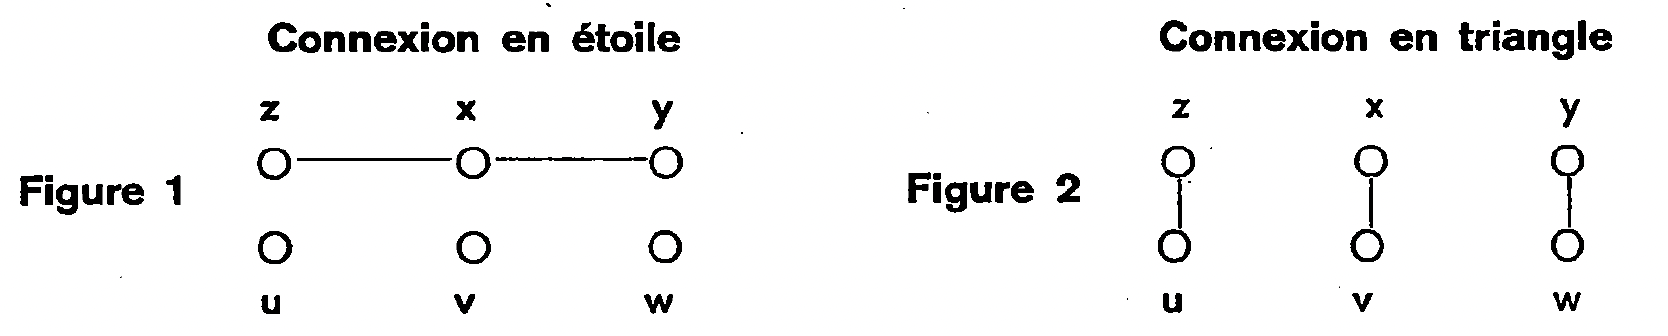
\includegraphics[width=1\linewidth]{images/page_64_motor_connections}
    \label{fig:schindler_motor_connections}
\end{figure}

To reverse the direction of rotation, it is sufficient to interchange two of the current supply wires at the terminal plate:

\begin{itemize}
    \item For three-phase motors: any two supply wires
    \item For two-phase motors with compound voltage: the two outer conductors
    \item For two-phase motors with non-compound voltage and single-phase motors: any two supply wires of the same phase
\end{itemize}

If the motor stops, it must be immediately disconnected. The maximum temperature should not exceed \(35^\circ C\) above
the ambient temperature. Refer to the diagram for details.

If the motor with a double-width pulley is intended for transmission with fixed and loose pulleys,
the belt must be on the loose pulley at startup and move to the fixed pulley only when the motor reaches its speed.

\section*{3. Maintenance}

The motor must be cleaned 1 or 2 times a year when it is out of operation, using a bellows or compressed air,
and then wiped with a cloth soaked in benzene. It is essential to avoid the penetration of oil or impurities into the winding.
Do not damage the insulation, and check if all terminals and nuts are securely tightened.

The sleeve bearings must be filled with oil as consumption occurs, and every 5 to 6 months, the oil must be renewed.
To prevent dust or dirt from falling into the bearings, wipe the covers before opening them. If necessary,
the bearings should be cleaned with petroleum.

Ball bearings consume very little grease, and one filling is expected to last for about 10,000 hours of operation.
After this period, but at least every 3 years, perform a new filling as follows:

